     \chapter{Zusammenfassung und Ausblick}
In diesem Projekt handelt es sich um eine Anwendung, die au�ergew�hnliche Situationen mit Hilfe einer Videokamera erkennen kann. Die Applikation orientiert sich an alten Menschen, die allein wohnen. Das Projekt ist eine Kombination von Hintergrundsubtraktion, Histogrammanalyse und Fuzzylogik. Im Rahmen dieser Arbeit wird ein Programm entwickelt, deren Eingaben sind die Bilder von einer 360� Grad Kamera sind. Das Programm mit Hilfe der Kamera beobachtet die Person im Alltag und gibt automatisch eine Meldung aus, wenn ein Unfall passiert. Das hat mich dazu motiviert, dieses Projekt zu entwickeln. \\

Ziel dieses Projekt ist die Entwicklung eine Anwendung, das Videos einer Bosch-360-Grad-Kamera verarbeitet. Das Programm soll eine Bewegung von einer Person erkennen, analysiert und Informationen geben, ob die Person in einer au�ergew�hnlichen Situation ist. Um eine abnormale Situation handelt es sich beispielsweise, wenn eine Person f�r l�ngere Zeit an einem Ort liegt. Um dieses Ziel zu realisieren, wurde das Programm aus drei gro�en Meilensteinen gebaut (Abbildung \ref{fig:zusammenfassung}). Der erste Meilenstein ist die Hintergrundsubtraktion. In diesem Schritt wird ein Bild als Eingabe mit einem Hintergrundbild verglichen. Der Unterschied zwischen Eingabebild und Hintergrundbild wird zuerst berechnet und ein Bin�rbild von dem Vordergrund wird danach zur�ckgeliefert. Eine Region der Bewegung wird mithilfe einer Begrenzungsbox beschr�nkt. Diese beschr�nkte Region wird in dem n�chsten Schritt ganz n�tzlich. Das Hintergrundbild wird immer nach Eingabe eines Bildes aktualisiert, wobei die  beschr�nkte Region nicht mit aktualisiert wird. Das hilft bei der Hintergrundsegmentierung, wenn die Person sich in der Szene nicht mehr bewegt. In dem zweiten Schritt wird die beschr�nkte Silhouette von dem letzten Schritt weiter analysiert, um die K�rperhaltung der Person zu erkennen. Die Silhouette wird zuerst von der Breite oder H�he auf 128 Pixel skaliert. Aus dem skalierten Bild werden vertikale und horizontale Histogramme gerechnet. Die Histogramme werden weiter mit Referenz-Histogrammen, die aus 4500 Silhouetten von 7 verschiedenen Personen mit 4 K�rperhaltungen (Liegen, Stehen, Beugen, Sitzen) berechnet wurden \cite{haritaoglu1998ghost}, verglichen. Nach dem Vergleichen wird die K�rperhaltung mit  einem maximalen Wert von Loglikelihood-Funktion ausgewertet. In letztem Schritt wird eine Fuzzymodell angewendet. Das Modell berechnet einfach wie hoch die Wahrscheinlichkeit ist, dass eine Person unter bestimmten Bedingungen in einer abnormalen Situation ist. Die Bedingung, die f�r einen abnormalen Fall erf�llt werden m�ssen, ist, wenn eine Person  auf dem Boden in einem vordefinierten Zeitraum (f�r Testen sind 30 Bildern aber das Parameter kann f�r spezielle F�lle modifiziert werden) liegt und sich nicht mehr bewegt. Ein Feature der Bosch-360-Grad Kamera ist die F�higkeit, in die Richtigen der Bewegung zu orientieren. Das wird auch in diesem Projekt verwendet und liefert nach Rotation des Kamerakopfes gleichbleibende Ergebnisse. \\
\begin{figure}[H]
	\centering
	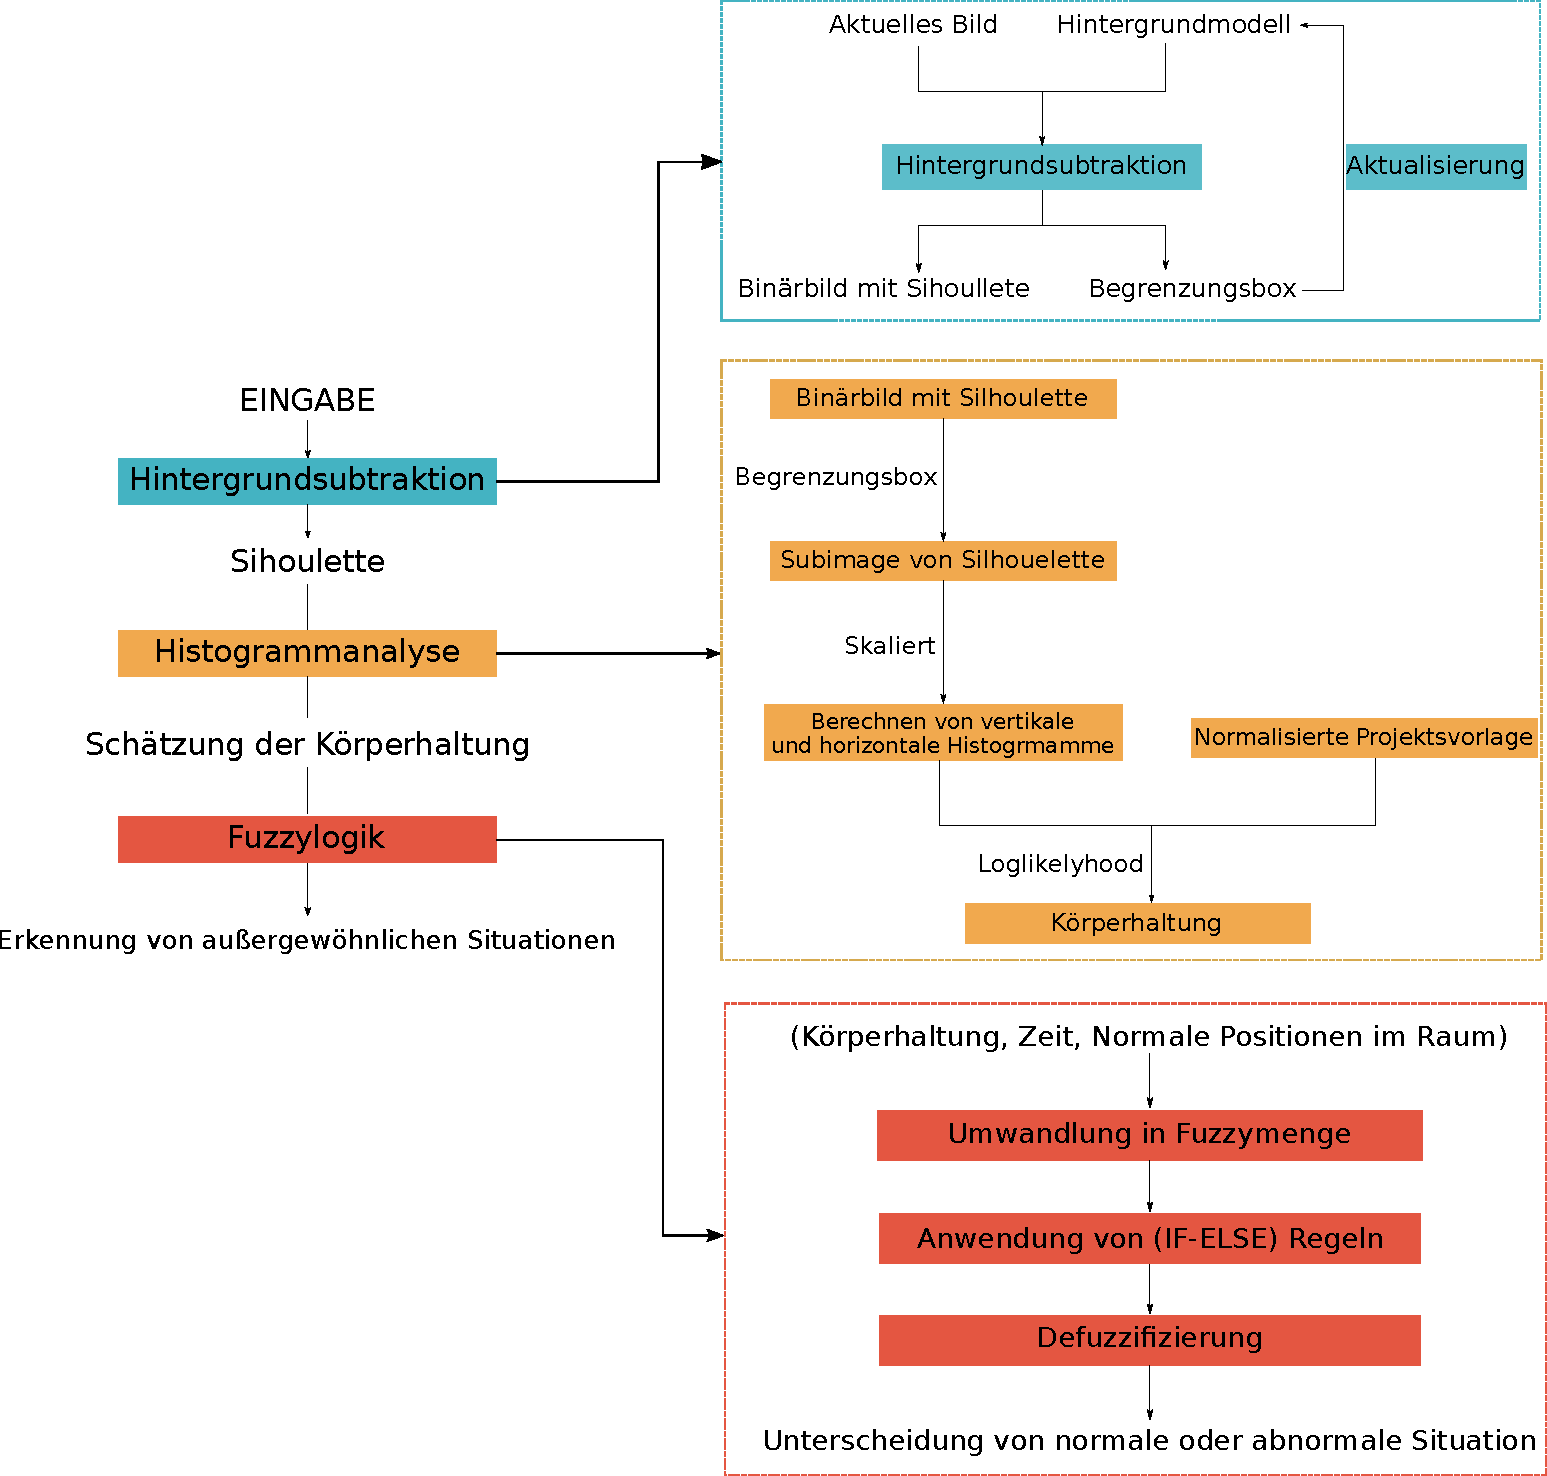
\includegraphics[width=1\textwidth]{fig/zusammenfassung.pdf}
	\caption{Zusammenfassung des Programmaufbaus}
	\label{fig:zusammenfassung}
\end{figure}
 Um die Ergebnisse von dem Projekt zu evaluieren, wird jedes Testvideos w�hrend der Teste annotiert. Die Testergebnisse wurden mit unseren erwartetet Werte verglichen. Das Programm kann alle au�ergew�hnlichen Situationen richtig erkennen und die K�rperhaltung der Person genau sch�tzen. Die Herausforderung der Arbeit besteht darin, die Verarbeitungszeit m�glichst gering zu halten. Bei einer durchschnittlichen Rechnerzeit von 109 Millisekunden pro Frame kann das Projekt als eine Echtzeitanwendung benutzt werden.\\
 
 Das Projekt hat viele Erweiterungspotenziale. Mir sind noch ein paar Ideen eingefallen, um das Programm noch umfangreicher zu machen.  Die erste Idee basiert auf der F�higkeit der Bewegungserkennung des Projektes. Die Kamera kann als ein Abwesenheitsmelder verwendet werden. Wenn es keine Bewegung in Haus in 24 Stunden gibt, dann wird eine Abwesenheitsmeldung ausgel�st oder ein Sicherheitsalarm wird automatisch angeschaltet. Meine zweite Idee ist eine Erweiterung des Projektes. Bis jetzt ist die Kamera noch nicht in die Smart Home App integriert. Wenn die Integration der Kamera mit der App realisiert wird, kann eine automatisch Lichtschaltung oder Heizungsschaltung sofort nach Erkennung einer Bewegung aktiviert werden. Die dritte Idee ist eine Verbesserung des Projektes. Heutzutage wird k�nstliche Intelligenz �berall verwendet. Mit Hilfe von neuronale Netz mit riesigem Datens�tzen kann die Sch�tzung der K�rperhaltung verbessert werden und damit wird die Qualit�t der Software auch deutlich erh�ht.